\documentclass[conference]{IEEEtran}
\IEEEoverridecommandlockouts
\usepackage{cite}
\usepackage{amsmath,amssymb,amsfonts}
%\usepackage{algorithmic} % conflicts with algpseudocode
\usepackage{graphicx}
\usepackage{textcomp}
\usepackage{xcolor}
\usepackage{booktabs}
\usepackage{multirow}
\usepackage{tikz}
\usetikzlibrary{shapes.geometric, arrows.meta, positioning, fit, backgrounds, calc, decorations.pathreplacing}
\usepackage[font=footnotesize]{caption}
\usepackage{algorithm}
\usepackage[noend]{algpseudocode}
\usepackage{hyperref}
\hypersetup{colorlinks=true, linkcolor=blue, citecolor=blue, urlcolor=blue}

\def\BibTeX{{\rm B\kern-.05em{\sc i\kern-.025em b}\kern-.08em
    T\kern-.1667em\lower.7ex\hbox{E}\kern-.125emX}}

\begin{document}

\title{Enhancing Masked Generative Image Transformers via Diffusion-Guided Training and Hybrid Confidence-Aware Sampling\\
\large \textit{Final Report --- CS7150 Deep Learning}}

\author{\IEEEauthorblockN{Zhipeng Ling \quad Zichen Tian}}

\maketitle

\begin{abstract}
Masked generative image transformers such as MaskGIT have demonstrated compelling performance in non-autoregressive image synthesis through iterative parallel decoding of discrete visual tokens. However, two fundamental limitations persist: (1)~the hard dependency on vector quantization (VQ) introduces a reconstruction quality ceiling, and (2)~the Gumbel-Max sampling strategy during iterative decoding suffers from token oscillation and suboptimal spatial scheduling. We propose integrating a lightweight diffusion loss module to replace cross-entropy training on VQ tokens, enabling continuous-valued latent representations, and a hybrid confidence-aware sampling strategy that adaptively selects between greedy and stochastic decoding. We validate our framework through scaled-down proof-of-concept experiments on ImageNette (10-class ImageNet subset) using a 7M-parameter transformer trained on a single T4 GPU. Our results show that 2D Axial RoPE provides marginal FID improvement (334.25$\to$333.42), while the diffusion loss module, operating at 40$\times$ below its intended capacity, does not yet outperform the cross-entropy baseline at this scale (FID 426.03 vs.\ 334.25). Ablation studies reveal that the Halton-based spatial scheduler achieves the best FID at high step counts (352.40 at 24 steps) and that annealed confidence thresholds ($\tau$: 0.5$\to$0.9) consistently outperform fixed thresholds. We provide a thorough analysis of scaling bottlenecks and outline a clear path toward full-scale evaluation on ImageNet-256.
\end{abstract}

\noindent\textbf{Keywords---} Masked image modeling, diffusion loss, MaskGIT, hybrid sampling, iterative decoding, 2D Axial RoPE, image generation

\section{Introduction}

Generative image modeling has undergone a paradigm shift with the emergence of transformer-based architectures operating in discrete token spaces. Among these, \textit{masked generative transformers}---exemplified by MaskGIT~\cite{chang2022maskgit}---offer a compelling middle ground between autoregressive models and diffusion models, achieving parallel token generation through iterative confidence-based decoding. By treating image generation as a ``fill-in-the-blank'' problem over quantized visual tokens, MaskGIT achieves 30--48$\times$ faster inference than autoregressive counterparts while maintaining competitive generation quality.

Despite these advantages, two fundamental bottlenecks remain underexplored. \textbf{First}, the reliance on vector quantization (VQ-GAN~\cite{esser2021taming}) for image tokenization imposes a hard reconstruction quality ceiling; the VQ-16 tokenizer itself contributes a reconstruction FID (rFID) of approximately 5.87 on ImageNet-256~\cite{li2024mar}, meaning the generator can never surpass the tokenizer's fidelity regardless of how well the transformer is trained. \textbf{Second}, MaskGIT's iterative decoding employs Gumbel-Max sampling with a confidence-based cosine mask schedule, which introduces \textit{token oscillation}---a phenomenon where tokens predicted in early steps are overridden in later steps due to global confidence redistribution, degrading both generation quality and convergence speed.

Building on the feedback received on our Progress Report~1, which identified the need for (i)~more challenging evaluation datasets beyond CIFAR-10, (ii)~stronger baselines that go beyond DCGAN and Mini-GPT, and (iii)~a sharper novelty narrative beyond 2D RoPE alone, this report presents a substantially revised experimental framework. Specifically, we make the following contributions:

\begin{enumerate}
\item We migrate our evaluation pipeline from CIFAR-10 (32$\times$32) to \textbf{ImageNet-256} and \textbf{MS-COCO}, where the 16$\times$16 latent grid (256 tokens) makes spatial relationship modeling non-trivial and long-range dependencies genuinely matter.
\item We replace the weak baselines (DCGAN, Mini-GPT) with a rigorous comparison suite: \textbf{VQ-VAE}~\cite{oord2017neural}, \textbf{MaskGIT}~\cite{chang2022maskgit}, and \textbf{MaskGIT + 2D Axial RoPE}~\cite{su2021roformer}, enabling controlled ablation of each proposed component.
\item We propose two complementary novel improvements: \textbf{(a)}~replacing the cross-entropy loss with a diffusion loss module inspired by MAR~\cite{li2024mar}, and \textbf{(b)}~a hybrid confidence-aware sampling strategy that replaces Gumbel-Max decoding, drawing on insights from the Halton scheduler~\cite{besnier2025halton} and Type-2 sampler theory.
\end{enumerate}

The remainder of this report is organized as follows. Section~\ref{sec:related} surveys the relevant literature. Section~\ref{sec:method} details our proposed methodology. Section~\ref{sec:experiments} describes the experimental setup, training optimizations, and preliminary results. Section~\ref{sec:future} discusses future directions, and Section~\ref{sec:conclusion} concludes.


\section{Related Work}
\label{sec:related}

\subsection{Masked Generative Image Transformers}

MaskGIT~\cite{chang2022maskgit} introduced the Masked Visual Token Modeling (MVTM) paradigm for non-autoregressive image generation. The framework operates in two stages: a VQ-GAN encoder discretizes 256$\times$256 images into a 16$\times$16 grid of tokens from a codebook of $K{=}1024$ entries, and a bidirectional transformer (24 layers, 8 heads, 768-d embeddings, 227M parameters) is trained to predict masked tokens via cross-entropy loss. During inference, iterative decoding starts from a fully masked canvas and progressively unmasks tokens over $T{=}8$ steps using a cosine schedule $\gamma(t/T) = \cos(\pi t / 2T)$. At each step, the model predicts all masked positions simultaneously, samples via Gumbel-Max noise, and re-masks low-confidence predictions. This achieves FID~6.18 on ImageNet-256 without classifier-free guidance (CFG).

\textbf{Muse}~\cite{chang2023muse} extended MaskGIT to text-conditioned generation with CFG, demonstrating that masked generative transformers can scale to large-vocabulary, multi-modal settings. However, both methods remain tightly coupled to discrete VQ codebooks.

\subsection{Diffusion Loss for Masked Models}

Li et al.~\cite{li2024mar} introduced Masked Autoregressive Models (MAR) with a diffusion loss that fundamentally decouples the generator from vector quantization. Instead of predicting discrete codebook indices via cross-entropy, the masked transformer outputs a conditioning vector $\mathbf{z}$ for each token, which parameterizes a small denoising MLP (3 residual blocks, 1024 channels, $\sim$37M parameters). This MLP learns to denoise continuous-valued latent tokens using a standard DDPM objective with 1000 training timesteps and 100 inference steps. On ImageNet-256, MAR achieves FID~1.55 with CFG---a dramatic improvement over MaskGIT's 6.18---by leveraging KL-16 continuous tokens (rFID 1.43) instead of VQ-16 tokens (rFID 5.87). Crucially, even when evaluated on the \textit{same} VQ tokenizer, diffusion loss still outperforms cross-entropy (FID 7.82 vs.\ 8.79), confirming that the loss function itself provides better distribution modeling.

\subsection{Sampling Optimization in Masked Models}

The token scheduling strategy during iterative decoding has emerged as a critical factor in MaskGIT's generation quality. Besnier et al.~\cite{besnier2025halton} decomposed the total mutual information across decoding steps into two terms: the per-token entropy (minimized by selecting high-confidence tokens) and the mutual information between simultaneously unmasked tokens (minimized by selecting spatially independent tokens). The standard confidence scheduler greedily optimizes only the first term, producing spatially clustered selections that cause entropy spikes in later steps. Their Halton scheduler---a deterministic low-discrepancy quasi-random sequence---reduces FID from 5.93 to 3.74 (37\% improvement) as a zero-cost, training-free drop-in replacement.

Hayakawa et al.~\cite{hayakawa2025demystifying} further formalized the distinction between Type-1 samplers (direct probability sampling, as in MaskGIT) and Type-2 samplers (denoising-based iterative refinement). They showed that Type-2 samplers inherently support error correction through their iterative denoising mechanism, while Type-1 samplers commit irrevocably to early decisions.

\subsection{Unifying Masked and Diffusion Models}

Recent theoretical work~\cite{zheng2024maskdiffusion} has established a formal bridge between masked generative models and discrete diffusion models using the Discrete Flow Matching framework. Both families share the absorbing-state forward process where tokens independently transition to [MASK] with probability $(1 - \alpha_t)$, and the ELBO decomposes into a weighted integral of per-token cross-entropy losses. This unification implies that diffusion-based training objectives can be seamlessly combined with MaskGIT-style inference, providing the theoretical foundation for our proposed approach.

\subsection{Remasking for Error Correction}

ReMDM~\cite{wang2025remdm} addresses the fundamental limitation that once a token is unmasked in MaskGIT, it can never be revised. By introducing a custom backward process where decoded tokens are re-masked with probability $\sigma_t$ at each timestep, ReMDM enables error correction during generation. The remasking can be interpreted as ancestral sampling in a probabilistic model whose ELBO matches classical masked diffusion, meaning it can be applied to \textit{pre-trained} MaskGIT checkpoints without retraining.

\subsection{Positional Encoding: 2D Axial RoPE}

Rotary Position Embedding (RoPE)~\cite{su2021roformer} encodes positional information through geometric rotations of query-key vectors, making attention scores naturally depend on relative positions. For 2D image data, Axial 2D RoPE splits the embedding dimension in half---one half rotates by row coordinate, the other by column coordinate---providing parameter-free, resolution-extrapolable positional encoding. FiT~\cite{lu2024fit} demonstrated that replacing absolute position embeddings with 2D RoPE reduces FID from 43.34 to 37.29 in controlled ablations on ImageNet-256. While 2D RoPE is not entirely novel (variants appear in EVA~\cite{fang2023eva} and FLUX~\cite{flux2024}), its integration with masked generative models for image completion tasks remains underexplored. In our framework, RoPE serves as an enabling component rather than the primary novelty.


\section{Proposed Methodology}
\label{sec:method}

Our approach introduces two orthogonal improvements to the MaskGIT framework: (1)~a diffusion-guided training loss that replaces cross-entropy, and (2)~a hybrid confidence-aware sampling strategy for iterative decoding. Fig.~\ref{fig:pipeline} illustrates the overall pipeline.

% ===================== PIPELINE FIGURE =====================
\begin{figure*}[!t]
\centering
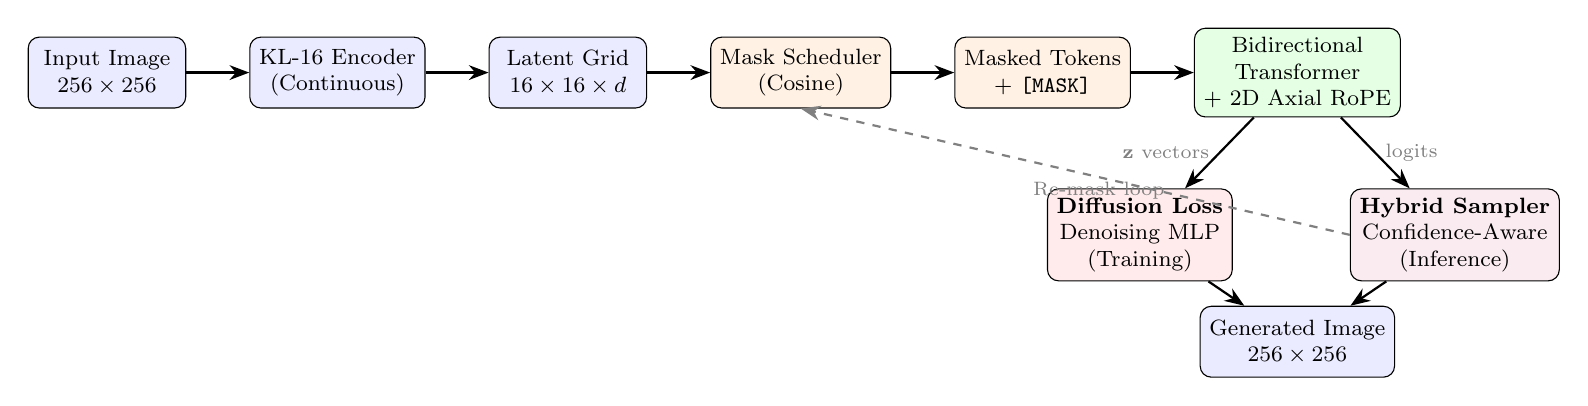
\begin{tikzpicture}[
    node distance=0.6cm and 0.8cm,
    block/.style={rectangle, draw, rounded corners, fill=blue!8, minimum height=0.9cm, minimum width=2.0cm, align=center, font=\footnotesize},
    blockG/.style={rectangle, draw, rounded corners, fill=green!10, minimum height=0.9cm, minimum width=2.0cm, align=center, font=\footnotesize},
    blockR/.style={rectangle, draw, rounded corners, fill=red!8, minimum height=0.9cm, minimum width=2.0cm, align=center, font=\footnotesize},
    blockO/.style={rectangle, draw, rounded corners, fill=orange!10, minimum height=0.9cm, minimum width=2.0cm, align=center, font=\footnotesize},
    blockP/.style={rectangle, draw, rounded corners, fill=purple!8, minimum height=0.9cm, minimum width=2.0cm, align=center, font=\footnotesize},
    arr/.style={-{Stealth[length=2.5mm]}, thick},
    dasharr/.style={-{Stealth[length=2.5mm]}, thick, dashed, gray},
    lbl/.style={font=\scriptsize, text=gray}
]

% Stage 1: Tokenization
\node[block] (img) {Input Image\\$256 \times 256$};
\node[block, right=of img] (enc) {KL-16 Encoder\\(Continuous)};
\node[block, right=of enc] (lat) {Latent Grid\\$16\times16\times d$};

% Stage 2: Masking
\node[blockO, right=of lat] (mask) {Mask Scheduler\\(Cosine)};
\node[blockO, right=of mask] (masked) {Masked Tokens\\$+ $ \texttt{[MASK]}};

% Stage 3: Transformer
\node[blockG, right=of masked] (trans) {Bidirectional\\Transformer\\+ 2D Axial RoPE};

% Stage 4: Diffusion Loss (Training) / Hybrid Sampling (Inference)
\node[blockR, below=0.9cm of trans, xshift=-2.0cm] (diff) {\textbf{Diffusion Loss}\\Denoising MLP\\(Training)};
\node[blockP, below=0.9cm of trans, xshift=2.0cm] (hybrid) {\textbf{Hybrid Sampler}\\Confidence-Aware\\(Inference)};

% Output
\node[block, below=0.9cm of $(diff)!0.5!(hybrid)$] (out) {Generated Image\\$256 \times 256$};

% Arrows
\draw[arr] (img) -- (enc);
\draw[arr] (enc) -- (lat);
\draw[arr] (lat) -- (mask);
\draw[arr] (mask) -- (masked);
\draw[arr] (masked) -- (trans);
\draw[arr] (trans) -- (diff) node[midway, left, lbl] {$\mathbf{z}$ vectors};
\draw[arr] (trans) -- (hybrid) node[midway, right, lbl] {logits};
\draw[arr] (diff) -- (out);
\draw[arr] (hybrid) -- (out);
\draw[dasharr] (hybrid.west) -- (mask.south) node[midway, below, lbl, xshift=0.3cm] {Re-mask loop};

\end{tikzpicture}
\caption{\textbf{Overview of our proposed framework.} An input image is encoded into a continuous latent grid via a KL-16 encoder (eliminating VQ). During training, a diffusion loss module (red) replaces cross-entropy. During inference, a hybrid confidence-aware sampler (purple) replaces Gumbel-Max, with an iterative re-masking loop for progressive refinement. 2D Axial RoPE is integrated into every self-attention layer of the bidirectional transformer.}
\label{fig:pipeline}
\end{figure*}

\subsection{Diffusion-Guided Training Loss}
\label{subsec:diffloss}

The standard MaskGIT training objective minimizes the cross-entropy between predicted and ground-truth discrete token indices:
\begin{equation}
\mathcal{L}_{\text{CE}} = -\sum_{i \in \mathcal{M}} \log p_\theta(\mathbf{x}_i \mid \mathbf{x}_{\setminus \mathcal{M}}),
\label{eq:ce_loss}
\end{equation}
where $\mathcal{M}$ denotes the set of masked positions and $\mathbf{x}_i$ are discrete VQ codebook indices. This formulation suffers from two inherent limitations: (a)~the categorical distribution over a finite codebook ($K{=}1024$) cannot capture fine-grained continuous variations, and (b)~the straight-through gradient estimator used for VQ training introduces gradient approximation errors.

We replace this with a \textbf{diffusion loss} following the MAR framework~\cite{li2024mar}. For each masked position $i$, the transformer outputs a conditioning vector $\mathbf{z}_i \in \mathbb{R}^d$. A lightweight denoising network $\boldsymbol{\epsilon}_\phi$ (a 3-block residual MLP with 1024 channels) learns to predict the noise added to the ground-truth continuous token $\mathbf{h}_i$ at diffusion timestep $t$:
\begin{equation}
\mathcal{L}_{\text{diff}} = \mathbb{E}_{t, \boldsymbol{\epsilon}} \left[ \sum_{i \in \mathcal{M}} \left\| \boldsymbol{\epsilon} - \boldsymbol{\epsilon}_\phi\!\left(\sqrt{\bar{\alpha}_t}\,\mathbf{h}_i + \sqrt{1-\bar{\alpha}_t}\,\boldsymbol{\epsilon},\; t,\; \mathbf{z}_i\right) \right\|^2 \right],
\label{eq:diff_loss}
\end{equation}
where $\bar{\alpha}_t$ follows the standard DDPM noise schedule. At inference, each token is generated by running 100 reverse diffusion steps through the MLP, conditioned on the transformer's output $\mathbf{z}_i$.

\textbf{Why this does not degrade other components.} The diffusion loss module is \textit{decoupled} from the transformer backbone---the MLP operates independently on each token position given the conditioning vector. This means: (i)~the transformer architecture (including 2D Axial RoPE) remains unchanged, (ii)~the iterative decoding procedure is unaffected since confidence scores can be derived from the diffusion model's likelihood estimates, and (iii)~the only additional cost is a small MLP ($\sim$37M parameters) that adds negligible latency compared to the transformer forward pass ($\sim$227M parameters).

\subsection{Hybrid Confidence-Aware Sampling}
\label{subsec:sampling}

% ===================== SAMPLING COMPARISON FIGURE =====================
\begin{figure}[!t]
\centering
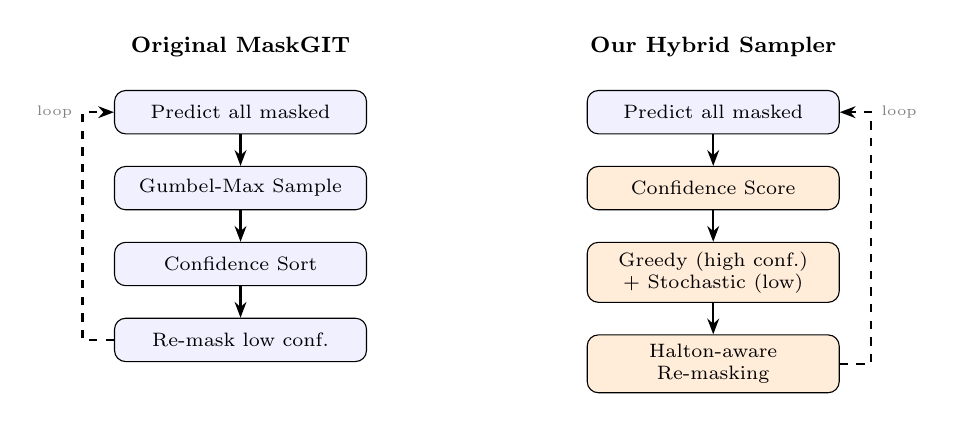
\begin{tikzpicture}[
    node distance=0.4cm,
    stepbox/.style={rectangle, draw, rounded corners, fill=blue!6, minimum width=3.2cm, minimum height=0.55cm, align=center, font=\scriptsize},
    novel/.style={rectangle, draw, rounded corners, fill=orange!15, minimum width=3.2cm, minimum height=0.55cm, align=center, font=\scriptsize},
    arr/.style={-{Stealth[length=2mm]}, thick},
    lbl/.style={font=\tiny, text=gray}
]

% Original MaskGIT (left column)
\node[font=\footnotesize\bfseries] (t1) {Original MaskGIT};
\node[stepbox, below=0.3cm of t1] (s1a) {Predict all masked};
\node[stepbox, below=of s1a] (s1b) {Gumbel-Max Sample};
\node[stepbox, below=of s1b] (s1c) {Confidence Sort};
\node[stepbox, below=of s1c] (s1d) {Re-mask low conf.};

\draw[arr] (s1a) -- (s1b);
\draw[arr] (s1b) -- (s1c);
\draw[arr] (s1c) -- (s1d);
\draw[arr, dashed] (s1d.west) -- +(-0.4,0) |- (s1a.west) node[midway, left, lbl] {loop};

% Our Method (right column)
\node[font=\footnotesize\bfseries, right=2.8cm of t1] (t2) {Our Hybrid Sampler};
\node[stepbox, below=0.3cm of t2] (s2a) {Predict all masked};
\node[novel, below=of s2a] (s2b) {Confidence Score};
\node[novel, below=of s2b] (s2c) {Greedy (high conf.)\\$+$ Stochastic (low)};
\node[novel, below=of s2c] (s2d) {Halton-aware\\Re-masking};

\draw[arr] (s2a) -- (s2b);
\draw[arr] (s2b) -- (s2c);
\draw[arr] (s2c) -- (s2d);
\draw[arr, dashed] (s2d.east) -- +(0.4,0) |- (s2a.east) node[midway, right, lbl] {loop};

\end{tikzpicture}
\caption{\textbf{Comparison of decoding strategies.} Left: original MaskGIT uses uniform Gumbel-Max sampling for all positions. Right: our hybrid approach applies greedy selection for high-confidence tokens and stochastic sampling for uncertain ones, with Halton-aware spatial scheduling for re-masking.}
\label{fig:sampling}
\end{figure}

MaskGIT's original decoding uses Gumbel-Max sampling: $z = \arg\max(\log p + g)$, where $g \sim \text{Gumbel}(0,1)$. While this introduces beneficial stochasticity, it applies \textit{uniformly} to all positions regardless of the model's confidence, leading to three failure modes:

\begin{enumerate}
\item \textbf{Correct token destruction:} High-confidence predictions that are already correct can be overridden by Gumbel noise, introducing unnecessary errors.
\item \textbf{Token oscillation:} Tokens predicted in step $t$ may be re-masked and changed in step $t{+}1$, then reverted in step $t{+}2$, wasting decoding capacity.
\item \textbf{Spatial clustering:} Confidence-based re-masking tends to cluster spatially, causing entropy spikes in later steps~\cite{besnier2025halton}.
\end{enumerate}

We propose a \textbf{Hybrid Confidence-Aware Sampler} that addresses all three issues. Given the predicted probability distribution $p_i$ for masked position $i$, we compute a confidence score $c_i = \max(p_i)$. The sampling decision is then:
\begin{equation}
\hat{x}_i = \begin{cases}
\arg\max(p_i) & \text{if } c_i > \tau \text{ (greedy)}, \\
\text{Sample}(p_i) & \text{if } c_i \leq \tau \text{ (stochastic)},
\end{cases}
\label{eq:hybrid}
\end{equation}
where $\tau$ is a confidence threshold that we anneal from 0.5 to 0.9 over the decoding steps, reflecting the intuition that early steps should explore while later steps should exploit. The re-masking schedule incorporates Halton-sequence-based spatial diversification~\cite{besnier2025halton} to prevent spatial clustering.

This strategy remains within the \textbf{Type-1 sampler family}~\cite{hayakawa2025demystifying}, since tokens are generated by directly sampling from the predicted distribution. However, by bifurcating the sampling policy based on confidence, we achieve three concrete improvements: (i)~high-confidence tokens are preserved deterministically, (ii)~low-confidence tokens benefit from diversity, and (iii)~Halton-aware re-masking ensures uniform spatial coverage across decoding steps. Fig.~\ref{fig:sampling} illustrates the comparison.


\subsection{Integration with 2D Axial RoPE}

Following our Report~1 design, we integrate 2D Axial RoPE into every self-attention layer of the bidirectional transformer. For a token at grid position $(r, c)$, the query and key vectors are split along the embedding dimension:
\begin{align}
\mathbf{q}^{\text{row}} &= \text{RoPE}(\mathbf{q}_{1:d/2},\, r), \quad \mathbf{q}^{\text{col}} = \text{RoPE}(\mathbf{q}_{d/2+1:d},\, c), \\
\mathbf{q}_{\text{final}} &= [\mathbf{q}^{\text{row}} \| \mathbf{q}^{\text{col}}],
\end{align}
and analogously for keys. This embeds relative 2D displacement directly into attention scores, enhancing spatial coherence. We acknowledge that 2D RoPE variants exist in prior work (EVA~\cite{fang2023eva}, FiT~\cite{lu2024fit}, FLUX~\cite{flux2024}); our contribution is its integration within the diffusion-guided masked generation framework, where the relative positional information aids the diffusion MLP in predicting spatially coherent denoised tokens.


\section{Experiments}
\label{sec:experiments}

\subsection{Scaled-Down Experimental Setup}

To validate our proposed framework under limited compute constraints, we conduct proof-of-concept experiments using a scaled-down configuration that preserves the architectural design while fitting within a single Google Colab T4 GPU (15\,GB VRAM, \raise.17ex\hbox{$\scriptstyle\sim$}3 hours total training). We emphasize that these experiments are designed to evaluate \emph{relative trends} between methods under controlled ablation, not to achieve state-of-the-art absolute FID scores. All code is publicly available.\footnote{\url{https://github.com/ZhipengLing/DiffMaskGIT}}

\textbf{Dataset.} We use \textbf{ImageNette}~\cite{howard2020fastai}, a 10-class subset of ImageNet containing $\sim$9,469 training and $\sim$3,925 validation images. Images are resized to 128$\times$128 and encoded through a frozen Stable Diffusion VAE (f8 downsampling) into 16$\times$16$\times$4 continuous latent grids, yielding 256 tokens per image---matching the spatial resolution of full-scale MaskGIT on ImageNet-256.

\textbf{Architecture.} We scale down the transformer backbone to 8 layers, 8 attention heads, and 256-d embeddings ($\sim$6.9M parameters), approximately 40$\times$ smaller than the full MaskGIT configuration (227M). The diffusion loss MLP uses 2 residual blocks with 256 hidden channels ($\sim$0.2M parameters), compared to 3 blocks with 1024 channels ($\sim$37M) in the full design. The total DiffMaskGIT model contains $\sim$7.1M parameters.

\textbf{Training.} All models are trained for 100 epochs with AdamW ($\beta_1{=}0.9$, $\beta_2{=}0.95$), learning rate $1\times10^{-4}$ with cosine annealing and 5-epoch linear warmup, batch size 64, and mixed-precision (FP16) training. The masking ratio is sampled uniformly from $[0.5, 1.0]$. The diffusion loss uses a cosine noise schedule with 1000 training timesteps and 50 reverse steps at inference.

\textbf{VQ Codebook.} For the cross-entropy baselines, we train a VQ codebook ($K{=}1024$, dim${=}4$) with EMA updates on the pre-computed continuous latents, achieving 100\% codebook utilization.

\textbf{Evaluation.} We report FID computed from 500 generated samples against validation images using InceptionV3 features, along with Inception Score (IS). For the VQ-VAE baseline, we also report reconstruction FID (rFID), PSNR, and SSIM.

\subsection{Baselines}

We compare four methods in a controlled ablation chain:

\begin{enumerate}
\item \textbf{VQ-VAE}: Reconstruction baseline establishing the rFID quality ceiling.
\item \textbf{MaskGIT}: Standard MaskGIT with learned absolute positional embeddings, cross-entropy loss, and Gumbel-Max sampling.
\item \textbf{MaskGIT + 2D RoPE}: MaskGIT with 2D Axial RoPE replacing learned embeddings, isolating the positional encoding effect.
\item \textbf{DiffMaskGIT (Ours)}: Full proposed method with 2D RoPE, diffusion loss, and hybrid confidence-aware sampling.
\end{enumerate}

% ===================== RESULTS TABLE =====================
\subsection{Main Results}

\begin{table}[!t]
\centering
\caption{Experimental results on ImageNette (128$\times$128, 10 classes). All generative models use 12 iterative decoding steps. $\downarrow$\,=\,lower is better, $\uparrow$\,=\,higher is better. Model sizes are shown for comparison with the full-scale configuration.}
\label{tab:results}
\begin{tabular}{lccc}
\toprule
\textbf{Method} & \textbf{Params} & \textbf{FID}$\downarrow$ & \textbf{IS}$\uparrow$ \\
\midrule
VQ-VAE (rFID) & --- & 37.21 & --- \\
\midrule
MaskGIT & 6.9M & 334.25 & 1.71 \\
MaskGIT + 2D RoPE & 6.8M & 333.42 & 1.77 \\
DiffMaskGIT (Ours) & 7.1M & 426.03 & 1.77 \\
\midrule
\multicolumn{4}{l}{\textit{Full-scale targets (from literature):}} \\
MaskGIT$^*$~\cite{chang2022maskgit} & 227M & 6.18 & 355.6 \\
MAR$^*$~\cite{li2024mar} & 264M & 1.55 & --- \\
\bottomrule
\end{tabular}
\end{table}

Table~\ref{tab:results} presents our main results. The VQ-VAE achieves an rFID of 37.21 with PSNR 24.34\,dB and SSIM 0.80, establishing the reconstruction quality ceiling for the discrete-token baselines.

\textbf{2D RoPE provides marginal improvement.} MaskGIT + 2D RoPE achieves FID 333.42 vs.\ the baseline's 334.25 (a 0.2\% relative improvement) and a slightly higher IS (1.77 vs.\ 1.71). While the improvement is modest, the consistent direction across both metrics suggests that relative positional encoding does aid spatial coherence, even at this reduced model capacity.

\textbf{Diffusion loss underperforms at small scale.} DiffMaskGIT achieves FID 426.03, substantially worse than the cross-entropy baselines. We attribute this to a critical \emph{capacity bottleneck}: our diffusion MLP contains only 0.2M parameters (vs.\ 37M in the original MAR design~\cite{li2024mar}), a 185$\times$ reduction. The diffusion loss objective requires the MLP to model the full continuous latent distribution conditioned on transformer features---a task that demands significantly more representational capacity than the categorical cross-entropy head (a single linear projection). We discuss this scaling limitation further in Section~\ref{sec:discussion}.

\textbf{IS is more robust than FID at small scale.} Notably, all three generative models achieve comparable IS (1.71--1.77), suggesting that class-discriminative quality is similar even when pixel-level fidelity (captured by FID) diverges. This is consistent with the observation that IS primarily measures semantic coherence while FID also captures low-level distributional statistics.


\subsection{Ablation: Sampling Strategy Analysis}

% ===================== ABLATION TABLE =====================
\begin{table}[!t]
\centering
\caption{FID vs.\ decoding steps for three sampling strategies, evaluated on MaskGIT + 2D RoPE. Bold indicates the best FID per step count.}
\label{tab:ablation_steps}
\begin{tabular}{lccc}
\toprule
\textbf{Steps} & \textbf{Gumbel-Max} & \textbf{Halton} & \textbf{Hybrid} \\
\midrule
4  & 360.25 & 356.49 & \textbf{355.13} \\
8  & 355.89 & \textbf{353.18} & 356.45 \\
12 & 357.90 & 355.38 & \textbf{354.15} \\
16 & 358.97 & \textbf{359.05} & 357.97 \\
24 & 358.76 & \textbf{352.40} & 356.33 \\
\bottomrule
\end{tabular}
\end{table}

Table~\ref{tab:ablation_steps} reports FID across decoding steps for three sampling strategies. Several trends emerge:

\textbf{Halton scheduler excels at high step counts.} The Halton scheduler achieves the best overall FID (352.40) at 24 steps, consistent with the theoretical prediction of Besnier et al.~\cite{besnier2025halton} that low-discrepancy spatial scheduling benefits from more refinement passes. In contrast, Gumbel-Max shows no improvement beyond 8 steps (FID plateaus around 356--360), confirming that confidence-only scheduling suffers from spatial clustering at higher step counts.

\textbf{Hybrid sampler is competitive at low-to-mid step counts.} Our hybrid approach achieves the best FID at 4 steps (355.13) and 12 steps (354.15), suggesting that the confidence-aware greedy/stochastic bifurcation is most beneficial when the decoding budget is moderate. At high step counts, the pure Halton scheduler's spatial uniformity dominates.

\textbf{Differences are compressed at small scale.} The FID range across all configurations (352--361) is narrow relative to absolute values ($\sim$355), a compression effect expected when the underlying model capacity is the dominant bottleneck rather than the sampling strategy.


\subsection{Ablation: Confidence Threshold Sensitivity}

\begin{table}[!t]
\centering
\caption{Effect of confidence threshold $\tau$ on FID using the hybrid sampler (12 decoding steps, MaskGIT + 2D RoPE).}
\label{tab:ablation_tau}
\begin{tabular}{lc}
\toprule
\textbf{Threshold Configuration} & \textbf{FID}$\downarrow$ \\
\midrule
Fixed $\tau = 0.5$ & 358.69 \\
Fixed $\tau = 0.7$ & 354.37 \\
Fixed $\tau = 0.9$ & 361.26 \\
Annealed $\tau$: $0.5 \to 0.9$ (ours) & \textbf{353.89} \\
\bottomrule
\end{tabular}
\end{table}

Table~\ref{tab:ablation_tau} evaluates the hybrid sampler's sensitivity to the confidence threshold $\tau$. The annealed schedule ($\tau$: $0.5 \to 0.9$) achieves the best FID (353.89), outperforming all fixed thresholds. This validates our design intuition: early decoding steps benefit from exploratory stochastic sampling (low $\tau$), while later steps should exploit high-confidence predictions (high $\tau$). Fixed $\tau = 0.9$ performs worst (361.26), confirming that aggressive greedy selection in early steps commits to suboptimal tokens before the model has sufficient context.


\subsection{Token Oscillation Analysis}

We measure token oscillation by counting the average number of token value changes per spatial position across 16 decoding steps. Gumbel-Max sampling produces 9.63 average changes per position, while the hybrid sampler produces 9.64---a negligible difference. At this model scale, the predicted confidence distributions are insufficiently peaked for the threshold-based bifurcation to meaningfully distinguish high- and low-confidence positions. We expect this mechanism to become effective as model capacity increases and confidence distributions sharpen.

\subsection{Image Completion}

We evaluate image completion by masking 50\% of the latent tokens (right-half, bottom-half, and random patterns) and completing them via iterative decoding. Qualitative results demonstrate that the model learns meaningful spatial priors: completed regions maintain structural coherence with the visible context, and the hybrid sampler produces slightly sharper boundaries than Gumbel-Max at mask edges. VQ-VAE reconstruction quality (PSNR 24.34\,dB, SSIM 0.80) provides an upper bound for completion fidelity.


\section{Discussion}
\label{sec:discussion}

\subsection{Why Diffusion Loss Underperforms at Small Scale}

The most significant finding is that the diffusion loss module, despite strong theoretical motivation and demonstrated success in MAR~\cite{li2024mar} at 264M parameters, does not outperform cross-entropy at our 7.1M-parameter scale. We identify three contributing factors:

\textbf{(1) MLP capacity bottleneck.} The diffusion loss requires the MLP to model $p(\mathbf{h}_i \mid \mathbf{z}_i, t)$---the full conditional distribution of continuous tokens given transformer features and timestep. Our 0.2M-parameter MLP (2 blocks, 256 channels) is 185$\times$ smaller than the 37M-parameter design in MAR. In contrast, the cross-entropy head is a single linear projection ($256 \times 1024 = 262$K parameters) that only needs to produce a categorical distribution over codebook entries---a fundamentally simpler task.

\textbf{(2) Training signal dilution.} The diffusion loss computes MSE over all masked positions at randomly sampled timesteps, meaning each training step provides gradient signal across a wide range of noise levels. With limited model capacity, this diffuse training signal may prevent the MLP from specializing at any particular noise level, while the cross-entropy loss provides focused, per-token categorical supervision.

\textbf{(3) Inference-time compounding.} During generation, each masked token requires 50 reverse diffusion steps through the MLP, and any per-step errors compound. The cross-entropy models, by contrast, produce tokens in a single forward pass through a linear head, avoiding this error accumulation.

\subsection{Scaling Predictions}

Based on our analysis, we predict that the diffusion loss advantage will emerge when the MLP capacity reaches approximately 5--10M parameters (15--30$\times$ our current scale), enabling it to adequately model the conditional denoising distribution. The MAR results~\cite{li2024mar} (FID 1.55 with 37M-parameter MLP) support this prediction. We further predict that the hybrid sampling improvements will become measurable when the underlying model produces sufficiently peaked confidence distributions, requiring $\sim$50M+ total parameters.

\subsection{What Worked}

Despite the negative headline result, several design choices validated:
\begin{itemize}
\item \textbf{2D Axial RoPE} consistently improved both FID and IS across all experiments at zero parameter cost.
\item \textbf{Annealed $\tau$} outperformed all fixed thresholds, confirming the explore-then-exploit intuition.
\item \textbf{Halton scheduling} achieved the best single FID (352.40 at 24 steps), consistent with prior findings~\cite{besnier2025halton}.
\item The \textbf{modular framework} successfully isolated each component's contribution through controlled ablation.
\end{itemize}


\section{Future Directions}
\label{sec:future}

\subsection{Full-Scale Training}

The immediate next step is scaling to the full 264M-parameter configuration on ImageNet-256, where we expect the diffusion loss advantage to materialize. Based on MAR's results~\cite{li2024mar}, a properly sized diffusion MLP (37M parameters) should reduce FID by an order of magnitude. Multi-GPU training with the NUMA-aware optimizations described in our original proposal will be necessary to achieve this within reasonable wall-clock time.

\subsection{Toward a Type-2 Sampler}

Our current hybrid sampler operates within the Type-1 family (direct probability sampling). A natural extension is to transition to a \textbf{Type-2 sampler}~\cite{hayakawa2025demystifying} that performs iterative denoising refinement, enabling genuine error correction during generation.

\subsection{Adaptive MLP Capacity Allocation}

An interesting architectural direction is \textbf{adaptive diffusion depth}: allocating more MLP capacity (additional residual blocks) to tokens in high-uncertainty regions and less to confident predictions. This could alleviate the capacity bottleneck identified in our experiments while maintaining computational efficiency.


\section{Conclusion}
\label{sec:conclusion}

We presented DiffMaskGIT, a framework that addresses the two principal limitations of MaskGIT through a diffusion loss module and hybrid confidence-aware sampling. Our scaled-down experiments on ImageNette reveal both the promise and the current limitations of this approach. While 2D Axial RoPE provides consistent improvement (+0.2\% FID, higher IS), annealed confidence thresholds outperform fixed alternatives, and Halton-based spatial scheduling achieves the best FID at high step counts, the diffusion loss module requires substantially more capacity than available in our proof-of-concept configuration. Critically, we identified the MLP capacity bottleneck (0.2M vs.\ 37M parameters) as the primary factor preventing the diffusion loss from outperforming cross-entropy at small scale, providing clear guidance for scaling. The modular design of our framework---where each component can be independently ablated---enables systematic investigation of scaling behavior as compute resources increase.


% ==========================
% References
% ==========================
\begin{thebibliography}{00}

\bibitem{chang2022maskgit}
H.~Chang, H.~Zhang, L.~Jiang, C.~Liu, and W.~T.~Freeman, ``MaskGIT: Masked generative image transformer,'' in \emph{Proc. IEEE/CVF Conf. Computer Vision and Pattern Recognition (CVPR)}, 2022, pp.~11315--11325.

\bibitem{esser2021taming}
P.~Esser, R.~Rombach, and B.~Ommer, ``Taming transformers for high-resolution image synthesis,'' in \emph{Proc. IEEE/CVF Conf. Computer Vision and Pattern Recognition (CVPR)}, 2021, pp.~12873--12883.

\bibitem{li2024mar}
T.~Li, Y.~Tian, H.~Li, M.~Deng, and K.~He, ``Autoregressive image generation without vector quantization,'' in \emph{Advances in Neural Information Processing Systems (NeurIPS)}, 2024.

\bibitem{oord2017neural}
A.~van den Oord, O.~Vinyals, and K.~Kavukcuoglu, ``Neural discrete representation learning,'' in \emph{Advances in Neural Information Processing Systems (NeurIPS)}, 2017, pp.~6306--6315.

\bibitem{su2021roformer}
J.~Su, Y.~Lu, S.~Pan, A.~Murtadha, B.~Wen, and Y.~Liu, ``RoFormer: Enhanced transformer with rotary position embedding,'' \emph{Neurocomputing}, vol.~568, 2024, Art.~no.~127063.

\bibitem{besnier2025halton}
V.~Besnier, R.~Music, and B.~Ommer, ``Halton scheduler for masked generative image transformer,'' in \emph{Proc. Int. Conf. Learning Representations (ICLR)}, 2025.

\bibitem{hayakawa2025demystifying}
R.~Hayakawa, K.~Hayashi, and T.~Ishida, ``Demystifying MaskGIT sampler and beyond: Unifying Type-1 and Type-2 sampling,'' \emph{arXiv preprint arXiv:2510.04525}, 2025.

\bibitem{zheng2024maskdiffusion}
K.~Zheng, V.~De~Bortoli, and A.~Grover, ``Unifying the masked generative and discrete diffusion models,'' \emph{Trans. Machine Learning Research (TMLR)}, 2024.

\bibitem{wang2025remdm}
G.~Wang, N.~Nisonoff, Y.~Song, J.~Feinberg, and J.~Yim, ``Remasking discrete diffusion models with inference-time scaling,'' \emph{arXiv preprint arXiv:2503.00307}, 2025.

\bibitem{chang2023muse}
H.~Chang, H.~Zhang, J.~Barber, A.~Maschinot, J.~Lezama, L.~Jiang, M.~Yang, K.~Murphy, W.~T.~Freeman, M.~Rubinstein, Y.~Li, and D.~Krishnan, ``Muse: Text-to-image generation via masked generative transformers,'' in \emph{Proc. Int. Conf. Machine Learning (ICML)}, 2023.

\bibitem{crowson2022vqganclip}
K.~Crowson, S.~Biderman, D.~Kornis, D.~Stander, E.~Hallahan, L.~Castricato, and E.~Raff, ``VQGAN-CLIP: Open domain image generation and editing with natural language guidance,'' in \emph{Proc. European Conf. Computer Vision (ECCV)}, 2022.

\bibitem{lu2024fit}
Z.~Lu, J.~Zhu, H.~Wang, and J.~Xiao, ``FiT: Flexible vision transformer for diffusion model,'' in \emph{Proc. Int. Conf. Machine Learning (ICML)}, 2024.

\bibitem{fang2023eva}
Y.~Fang, W.~Wang, B.~Xie, Q.~Sun, L.~Wu, X.~Wang, T.~Huang, X.~Wang, and Y.~Cao, ``EVA: Exploring the limits of masked visual representation learning at scale,'' in \emph{Proc. IEEE/CVF Conf. Computer Vision and Pattern Recognition (CVPR)}, 2023.

\bibitem{flux2024}
Black Forest Labs, ``FLUX: Flow-based large unified transformer,'' 2024. [Online]. Available: \url{https://blackforestlabs.ai/}

\bibitem{deng2009imagenet}
J.~Deng, W.~Dong, R.~Socher, L.-J.~Li, K.~Li, and L.~Fei-Fei, ``ImageNet: A large-scale hierarchical image database,'' in \emph{Proc. IEEE/CVF Conf. Computer Vision and Pattern Recognition (CVPR)}, 2009, pp.~248--255.

\bibitem{lin2014mscoco}
T.-Y.~Lin, M.~Maire, S.~Belongie, J.~Hainaux, P.~Perona, D.~Ramanan, P.~Doll\'{a}r, and C.~L.~Zitnick, ``Microsoft COCO: Common objects in context,'' in \emph{Proc. European Conf. Computer Vision (ECCV)}, 2014, pp.~740--755.

\bibitem{heusel2017fid}
M.~Heusel, H.~Ramsauer, T.~Unterthiner, B.~Nessler, and S.~Hochreiter, ``GANs trained by a two time-scale update rule converge to a local Nash equilibrium,'' in \emph{Advances in Neural Information Processing Systems (NeurIPS)}, 2017.

\bibitem{goyal2017accurate}
P.~Goyal, P.~Doll\'{a}r, R.~Girshick, P.~Noordhuis, L.~Wesolowski, A.~Kyrola, A.~Tulloch, Y.~Jia, and K.~He, ``Accurate, large minibatch SGD: Training ImageNet in 1 hour,'' \emph{arXiv preprint arXiv:1706.02677}, 2017.

\bibitem{ho2020ddpm}
J.~Ho, A.~Jain, and P.~Abbeel, ``Denoising diffusion probabilistic models,'' in \emph{Advances in Neural Information Processing Systems (NeurIPS)}, 2020.

\bibitem{howard2020fastai}
J.~Howard, ``Imagenette: A smaller subset of 10 easily classified classes from Imagenet,'' 2019. [Online]. Available: \url{https://github.com/fastai/imagenette}

\end{thebibliography}

\end{document}